\appendix


\chapter{Introdução à geoestatística multivariada}

Em muitos casos os problemas relacionados com a estimativa de uma variável de interesse estão associados com duas ou mais variáveis. A geoestatística multivariada é o conjunto de técnicas que permite avaliar concomitantemente  mais de uma variável de forma a criar estimativas que incorporem informações diferentes, mas correlacionadas. 

Quando realizamos estimativas de variáveis aleatórias diferentes utilizando krigagem ordinária, tal como teores de um dado minério, ocorre a presença de erros de fechamento. Ou seja, se um minério contendo apenas ferro e quartzo em proporções de 60$\%$ e 40$\% $ não há garantias que as krigagens individuais permanençam com estas proporções. No entanto, utilizando a cokrigagem, por exemplo, conseguimos estimar mantendo as proporções individuais de cada elemento no minério. 

Outra utilização da geoestatística multivariada é a incorporação de amostras com suporte diferenciado. Em muitos casos nas campanhas de pesquisa coexistem amostras retiradas por métodos diferenciados tais como sondagem diamantada e pó de perfuratriz. Essas amostras não podem ser utilizadas juntamente pois apresentam precisões e qualidades diferentes e volumes também diferenciados. Utilizando a geoestatística multivariada podemos tratar uma outra informação como uma variável secundária e acrescentar informação que pode qualificar melhor nossa variável de interesse. 

Em alguns casos a geoestatística multivariada tem valor muito mais preponderante do que a geoestatística univariada. Em poços de petróleo, em que as informações primárias são escassas, a geofísica de reflexão tem um papel muito mais importante na incorporação da informação na estimativa.

A geoestatística multivariada, tal como a geoestatística convencional, tem os mesmos objetivos principais, mas que, no entanto, se caracterizam pela utilização de múltiplas entradas do modelo. A descrição, interpretação e estimativa são realizadas de forma muito mais complexa e interdependente.  
Como todo modelo, naturalmente ela não envolverá toda a gama possível de variações e situações encontradas, pois é de fato uma simplificação da realidade. Ao adotarmos a geoestatística convencional, colocamos sob julgamento uma variável objetivo independente de qualquer outro fator,  que caracterizará por todo o processo de decisão.  A krigagem ordinária, por exemplo, tem como variável independente as amostras situadas em cada local, e como resposta o valor médio desta variável em um ponto considerado. Mas nada indica que esta variável dependente é apenas condicionada a uma única variável.  Tomemos como exemplo um problema físico, demonstrado em \eqref{bola_canhao}, em que o objetivo é determinar o ponto de parada de uma bola de canhão. Se desconsiderarmos o efeito da resistência do ar, a posição da bola será apenas dependente da velocidade inicial. O modelo inicial é mais simples, mas não garantirá boa precisão, mas se incorporarmos uma variável correlata tal como a resistência do ar, o modelo se tornará mais fiel e semelhante com a realidade. De fato nunca haverá modelo que consiga se acercar de todas as possibilidades de variação, mas cada modelo mais robusto caracterizará melhor as incertezas do problema. 
 
\begin{figure}[H]
	\centering
	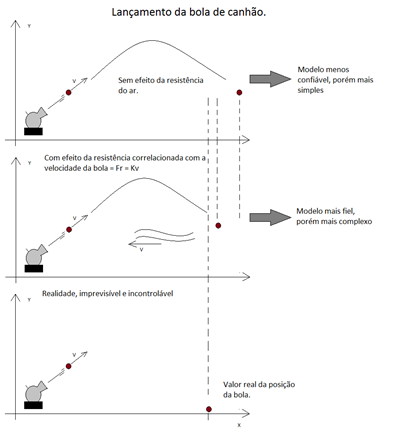
\includegraphics[scale=1.0]{bola.png}	
	\caption{Modelos físicos diferentes produzindo diferentes resultados. Incerteza sempre dependente do modelo escolhido}
	\label{bola_canhao}
\end{figure}

\section{Modelos multivariados}

Dentre as metodologias mais comuns de geoestatística multivariada temos:

\begin{itemize}
	\item Krigagem simples com médias locais variáveis 
	\item Krigagem com deriva externa 
	\item Cokrigagem ordinária 
	\item Cokrigagem colocada
\end{itemize}

Existem vários outros modelos geoestatísticos multivariados disponibilizados. Para maiores informações procurar "Geoestatistical for Natural Resources Evaluation" - Pierre Goovaerts. 

\subsection{Krigagem simples com médias locais variáveis}

Como notação para a geoestatística multivariada neste livro mudaremos a notação geralmente utilizada de $Z(x_{i})$ para indicar uma variável aleatória no ponto i e mudaremos para $Z_{j}(x_{i})$ tal que j é o índice da variável para o ponto i no espaço.

Lembrando do estimador da krigagem simples tínhamos a equação \eqref{KrigSimples} representando a estimativa em um ponto desconhecido:

\begin{equation}\label{KrigSimples}
	 Z^*(x_0) = \sum_{i=0}^{n} \lambda_{i}\left( Z(x_i) - m \right) + m
\end{equation}

Segundo a hipótese de estacionaridade de segunda ordem o valor de m não depende da posição no espaço sendo um valor constante ao longo de todo o domínio. Podemos utilizar a informação secundária para inferir o valor da média m no ponto desconhecido segundo uma regressão linear. Logo temos a equação da krigagem simples com médias locais variáveis descritas por \eqref{KrigSimples2}:

\begin{equation}\label{KrigSimples2}
Z^*_{j}(x_0) = \sum_{i=0}^{n} \lambda_{i}\left( Z_{j}(x_i) - msk \right) + msk
\end{equation}
 
 Em que msk é a média regredida entre uma variável j de interesse e uma outra variável qualquer. 
 
 \subsection{Krigagem com deriva externa}
 
 Na krigagem com deriva externa não estamos interessados em substituir as médias locais por uma estimativa obtida por regressão linear. Na verdade, neste caso, estamos interessados apenas no modelo a ser utilizado para estas médias. 
 
 Geralmente o modelo utilizado para calcular a tendência da função aleatória são polinômios de graus diferenciados. Neste caso a forma mais simples é um modelo linear tal que temos o valor médio igual a $m(x_{i}) = A Z_2(x_{i}) + B$, sendo os coeficientes A e B implicitamente calculados pela matriz de krigagem e $Z_2$ é a variável aleatória secundária. Neste caso o polinômio pode ser caracterizado como uma soma de funções tal que $\sum_{j=0}^{p} a_{j} fy_{j}$ sendo p o grau máximo do polinômio e as funções fy sendo os expoentes das variáveis, ou seja $a_1 y_1 + a_2 y^2_2 + ... + a_n y^n_n$.
 
Logo o sistema de krigagem simples pode ser determinado por \eqref{eq1}: 
 
\begin{equation} \label{eq1}
	Z_{j}(x_{0}) = \sum_{j=0}^{p} a_{j} fy_j(x_0) + \sum_{i=0}^{n}\lambda_{i}\left[ Z_j(x_{i}) - \sum_{j=0}^{p} a_{j} fy_j(x_i)\right]
\end{equation}
 
 Em que $a_j$ são os coeficientes constantes do problema e $fy_j(x_i)$ é o expoente do polinômio no ponto i considerado. Podemos então simplificar a equação acima separando apenas os coeficientes do polinômio, logo podemos ter a equação 
 
 \begin{equation} \label{eq2}
 Z_{j}(x_{0}) = \sum_{i=0}^{n}\lambda_{i}Z_j(x_{i})  + \sum_{j=0}^{p} a_{j}\left[fy_j(x_0) -\sum_{i=0}^{n}\lambda_{i}fy_j(x_i) \right]
 \end{equation}
 
Impondo a restrição que o valor da variável secundária no ponto estimado deve ser igual à uma combinação linear dos valores da variável secundária na região mais próxima temos uma resolução não enviesada do problema tal que:

\begin{equation} \label{eq3}
\sum_{j=0}^{p} a_{j}\left[fy(x_0) -\sum_{i=0}^{n}\lambda_{i}fy(x_i) \right] = 0
\end{equation} 
 
Temos então que:

\begin{equation} \label{eq4}
  fy(x_0) = \sum_{i=0}^{n}\lambda_{i}fy(x_i)
\end{equation}

Logo o sistema de krigagem nada mais é do que similarmente um sistema de krigagem simples com a restrição dada pela equação \eqref{eq4}. Para utilizar, no entanto, essa metodologia precisamos ter a variável secundária medida extensivamente. Isso significa que em cada local que estimarmos o valor da variável primária é necessário haver uma medida da variável secundária no ponto a ser estimado e nos pontos utilizados para a estimativa.  

A matriz de krigagem fica então modificada para \eqref{eq5}: 


\begin{equation}\label{eq5}
\begin{pmatrix}
Cov(Y_{1},Y_{1})&Cov(Y_{1},Y_{2})& ... & Cov(Y_{1},Y_{n})& fy(x_1)\\ 
Cov(Y_{2},Y_{1})&Cov(Y_{2},Y_{2})& ... & Cov(Y_{2},Y_{n})& fy(x_2) \\ 
...&...& ...&... & ...\\
Cov(Y_{n},Y_{1})&Cov(Y_{n},Y_{2})& ... & Cov(Y_{n},Y_{n})& fy(x_n)\\
1&1& ...&1& 0\\
fy(x_1)&fy(x_2)& ...&fy(x_n)& 0
\end{pmatrix} 
\begin{pmatrix}
\lambda _{1}\\ 
\lambda _{2}\\ 
...\\ 
\lambda _{n}\\
1/2\mu
\end{pmatrix}=\begin{pmatrix}
Cov(Y_{0}, Y_{1})\\ 
Cov(Y_{0}, Y_{2})\\  
...\\
Cov(Y_{0}, Y_{n})\\
1\\
fy(x_0)
\end{pmatrix}
\end{equation}

 \subsection{Cokrigagem }
 
 Diferentemente da krigagem a cokrigagem utiliza diversas variáveis aleatórias em uma combinação linear de forma a produzir a melhor solução no ponto estimado. A equação \eqref{eq6} demonstra como o ponto $ Z(x_{0})$ pode ser estimado a partir de uma combinação de variáveis aleatórias j:

\begin{equation}\label{eq6}
	Z_{j}(x_{0}) = \sum_{j=0}^{p}\sum_{i=0}^{n}\lambda^{j}_{i} Z_{j}(x_{i})\forall j
\end{equation}

Podemos então determinar a variância de extensão da cokrigagem como demonstrado na equação \eqref{eq7}

\begin{equation}\label{eq7}
\sigma^2_{ext} = E\left( Z_{j} (x_{0}) - \sum_{j=0}^{p}\sum_{i=0}^{n} \lambda^j_{i} Z_j(x_{i})\right)^2
\end{equation}

Para encontrarmos a matriz de krigagem devemos realizar a expansão da equação \eqref{eq7} anterior, tomar o valor esperado de cada termo encontrando as covariâncias e realizar a derivada parcial em relação a cada índice i e j, sendo i o número da amostra e j o número da variável considerada. Observamos na demonstração abaixo que :

 
\begin{proof}
	 $E\left( Z_{j} (x_{0}) - \sum_{j=0}^{p}\sum_{i=0}^{n} \lambda^j_{i} Z_j(x_{i})\right)^2$
	 \\
	 $E\left( (Z_{j} (x_{0}))^2 -2\sum_{j=0}^{p}\sum_{i=0}^{n} \lambda^j_{i} Z_j(x_{i})Z^*_{j} (x_{0}) + \sum_{j=0}^{p}\sum_{i=0}^{n} \sum_{j'=0}^{p}\sum_{i'=0}^{n}\lambda^j_{i}\lambda^{j'}_{i'} Z_j(x_{i})Z_{j'}(x_{i'})  \right)$
	 \\
	 Tomando a esperança matemática de cada parcela temos
	 \\
	 $Cov(Z_{j} (x_{0}),Z_{j} (x_{0}) ) -2\sum_{j=0}^{p}\sum_{i=0}^{n} \lambda^j_{i} Cov(Z_j(x_{i}),Z^*_{j} (x_{0})) + \\ \sum_{j=0}^{p}\sum_{i=0}^{n} \sum_{j'=0}^{p}\sum_{i'=0}^{n}\lambda^j_{i}\lambda^{j'}_{i'} Cov(Z_j(x_{i}),Z_{j'}(x_{i'}))$\\
	 Tomando a derivada parcial em relação a cada $\lambda^j_{i} \forall i,j$ temos que:
	 \\
	 $Cov(Z_{j}(x_{i}),Z_{j} (x_{0}))=\sum_{j'=0}^{p}\sum_{i'=0}^{n}\lambda^{j'}_{i'}Cov(Z_j(x_{i}),Z_{j'}(x_{i'})) \forall i,j$
\end{proof}

Esse sistema de krigagem tende a aumentar cada vez mais com a incorporação de mais variáveis secundárias.A figura \eqref{cokrig} demonstra um exemplo gráfico das partições da matriz de cokrigagem.Neste caso, diferentemente da matriz de krigagem que temos apenas as covariâncias diretas entre ponto a ponto, temos também as variâncias cruzadas.

\begin{figure}[H]
	\centering
	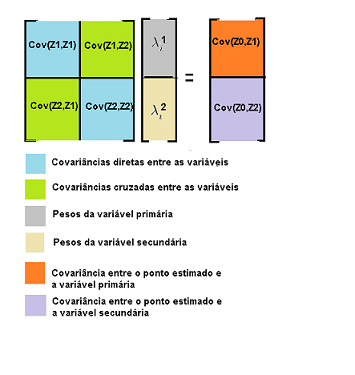
\includegraphics[scale=1.0]{cokrig.png}	
	\caption{Demonstração da matriz de cokrigagem para duas variáveis. Diferentes cores identificam as componentes da matriz}
	\label{cokrig}
\end{figure} 

Como demonstrado no capítulo de variografia os covariogramas cruzados não necessariamente são funções pares, e como consequência simétricas. Efeitos de delay podem prejudicar na modelagem de covariogramas sendo a opção de variogramas cruzados a melhor alternativa para a utilização de um modelo linear de corregionalização. 

A utilização da cokrigagem não requer que os dados estejam colocados tal como na krigagem com deriva externa. No entanto é necessário determinar um modelo linear de corregionalização de forma a ser capaz a utilização do método. Isso torna a metodologia muito trabalhosa e nem sempre adotada pela maioria dos modeladores exigindo simplificações tais como a utilização de modelos markovianos. 
  
 \subsection{Influência dos dados secundários}
 
A influência dos dados secundários na estimativa da variável primária depende dos seguintes fatores:

\begin{itemize}
	\item A correlação entre a variável primária e a secundária 
	\item A forma da continuidade espacial entre as variáveis 
	\item A configuração espacial entre as variáveis primárias e secundárias 
	\item a densidade amostral de cada variável 
\end{itemize} 

Nota-se que a variável secundária tende a ter maior importância quanto maior for o coeficiente de correlação e menor o efeito pepita relativo entre a variável secundária e a primária. Quanto maior for a qualidade das amostras, ou seja maior acurácia, melhor serão os resultados provenientes da cokrigagem. 

 \subsection{Condição não tradicional e tradicional da cokrigagem}
 
 Sob a condição tradicional de não enviesamento, espera-se que o sistema de resolução das equações incorpore duas condições de contorno tal que a soma dos pesos de cokrigagem da variável primária seja iguais a 1 e das secundárias seja igual a zero. Essa alternativa é feita para que a variável secundária apenas modifique os pesos de krigagem mas não as unidades do valor estimado. A condição não tradicional, no entanto, propõe que a soma das duas condições seja igual a 1. 
 
 \subsection{Cokrigagem Colocada}
 
 A cokrigagem colocada é uma simplificação da cokrigagem convencional, ao qual utilizada dados densamente amostrados para o cálculo dos valores estimados. Na cokrigagem colocada apenas os valores da variável secundária no local onde será estimado o valor da variável aleatória é utilizado.  A simplificação permite constatar que a influência da variável secundária é proporcional à distância do ponto estimado, logo ao utilizar a variável apenas no local estimado seu valor "blinda" a influência dos valores mais próximos. Essa condição se torna cada vez mais verdadeira se a correlação entre a variável primária e a secundária tende a ser maior.  

 